\documentclass[xetex,mathserif,serif]{beamer}
\usepackage{polyglossia}
\setdefaultlanguage[babelshorthands=true]{russian}
\usepackage{minted}
\usepackage{tabu}
\usepackage[11pt]{moresize}

\useoutertheme{infolines}

\usepackage{fontspec}
\setmainfont{FreeSans}
\newfontfamily{\russianfonttt}{FreeSans}

\usepackage{textpos}
\setlength{\TPHorizModule}{1cm}
\setlength{\TPVertModule}{1cm}

\definecolor{links}{HTML}{2A1B81}
\hypersetup{colorlinks,linkcolor=,urlcolor=links}

\tabulinesep=0.7mm

\title{Архитектурные аспекты сетевой безопасности}
\subtitle{Часть 2: Аутентификация}
\author[Юрий Литвинов]{Юрий Литвинов \newline \textcolor{gray}{\small\texttt{yurii.litvinov@gmail.com}}}

\newcommand{\attribution}[1] {
\vspace{-5mm}\begin{flushright}\begin{scriptsize}\textcolor{gray}{\textcopyright\, #1}\end{scriptsize}\end{flushright}
}

\date{27.05.2019г}

\begin{document}

	\frame{\titlepage}

	\section{Квантовая криптография}

	\begin{frame}
		\frametitle{Квантовый шифр}
		\framesubtitle{Протокол Bennett-Brassard BB84}
		\begin{center}
			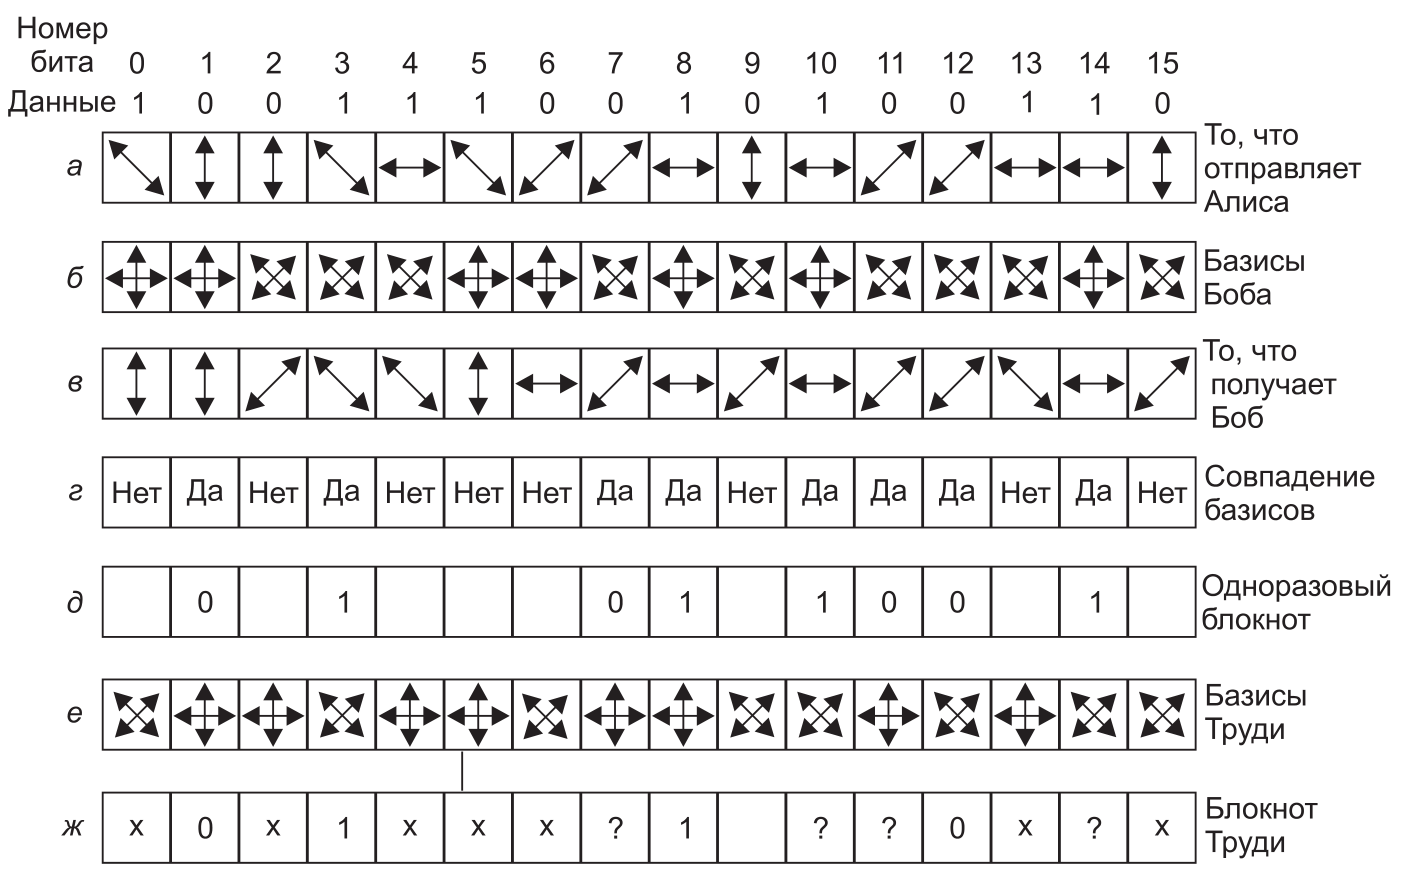
\includegraphics[width=0.9\textwidth]{quantumCipher.png}
			\attribution{Э. Таненбаум}
		\end{center}
	\end{frame}

	\section{Сертификаты}

	\begin{frame}
		\frametitle{Сертификаты}
		\begin{center}
			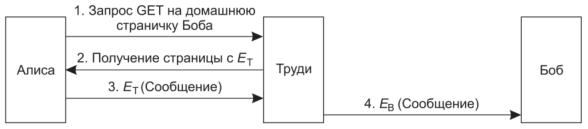
\includegraphics[width=0.6\textwidth]{manInTheMiddle.png}
			\attribution{Э. Таненбаум}
		\end{center}
		\begin{itemize}
			\item Сертификат --- сообщение, подтверждающее идентичность ключа, подписанное Certificate Authority (стандарт X.509)
			\item Цепочка сертификатов --- CA верхнего уровня подписывает сертификаты CA уровнем ниже, чтобы они могли подписывать сертификаты пользователей
			\item Корневые сертификаты --- сертификаты, которым принято доверять
			\item Самоподписанные сертификаты --- не доверенные, используются для отладки
		\end{itemize}
	\end{frame}

	\begin{frame}
		\frametitle{Применения сертификатов}
		\begin{itemize}
			\item Протокол HTTPS, проверка идентичности сервера
			\item Подписывание кода (Windows SmartScreen, Apple Code Signing)
			\item Подписывание сборок, сильные имена сборок в .NET
		\end{itemize}
		\begin{center}
			\includegraphics[width=0.6\textwidth]{dotNetCodeSigning.png}
			\attribution{J. Richter}
		\end{center}
	\end{frame}

	\begin{frame}
		\frametitle{Сертификаты (2)}
		\begin{center}
			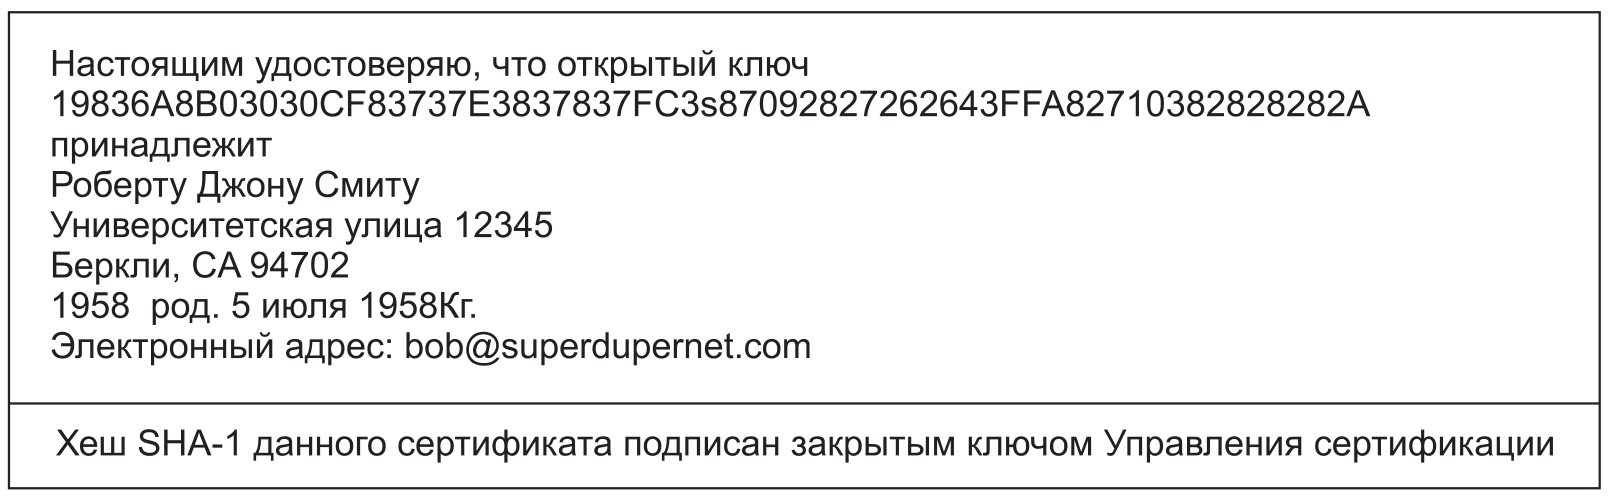
\includegraphics[width=0.75\textwidth]{certificate.png}
			\attribution{Э. Таненбаум}
		\end{center}
		\begin{itemize}
			\item Подписанный у CA сертификат стоит денег (от \$7 до более \$200 в год, в зависимости от типа)
			\begin{itemize}
				\item И требует идентификации личности (по паспорту или чему-то такому)
			\end{itemize}
			\item Сертификаты всегда выдаются на фиксированное время
			\item Сертификат можно отозвать
			\item Куча несовместимых форматов: .pem, .p12, .pfx, .der, .cer, .crt
		\end{itemize}
	\end{frame}

	\begin{frame}
		\frametitle{Certificate Authority}
		\begin{center}
			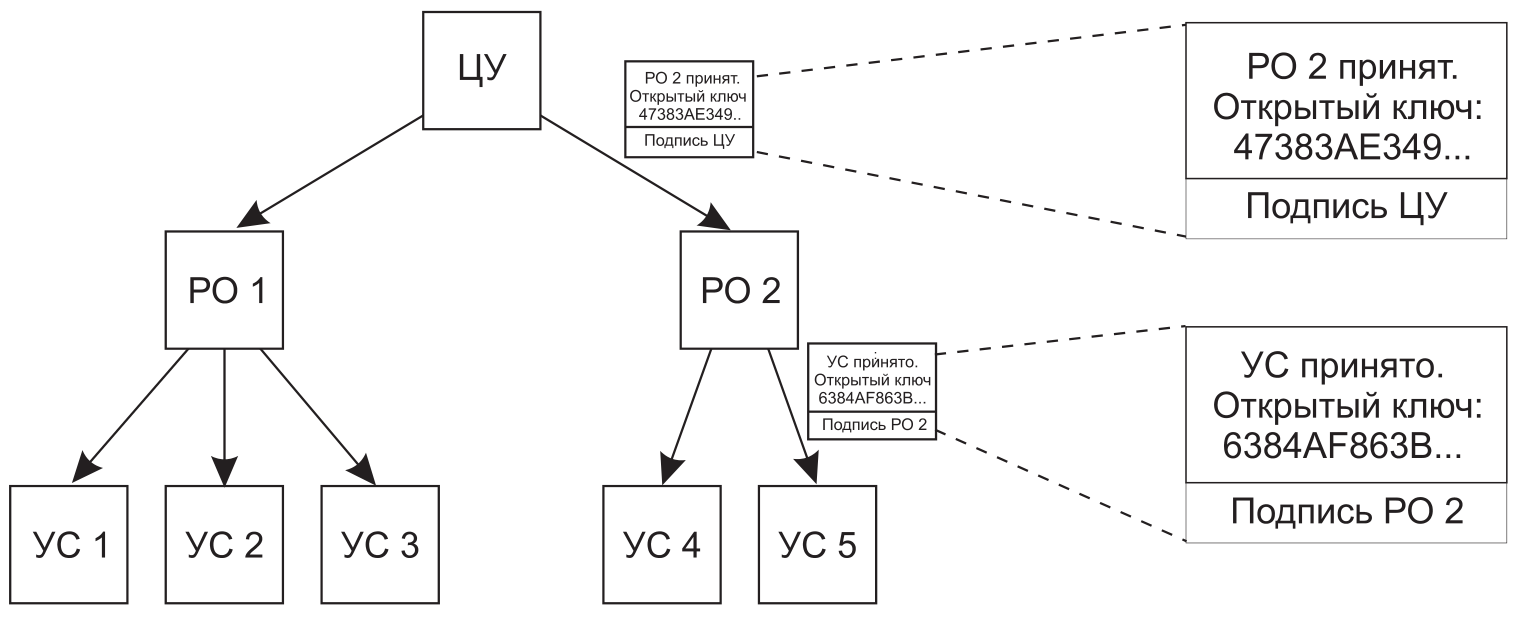
\includegraphics[width=0.85\textwidth]{certHierarchy.png}
			\attribution{Э. Таненбаум}
		\end{center}
		\begin{itemize}
			\item \url{https://letsencrypt.org/} --- автоматически и бесплатно даёт сертификаты, но им почти никто не доверяет
		\end{itemize}
	\end{frame}

	\begin{frame}
		\frametitle{Менеджер сертификатов, Windows}
		\framesubtitle{Snap-In в MMC}
		\begin{center}
			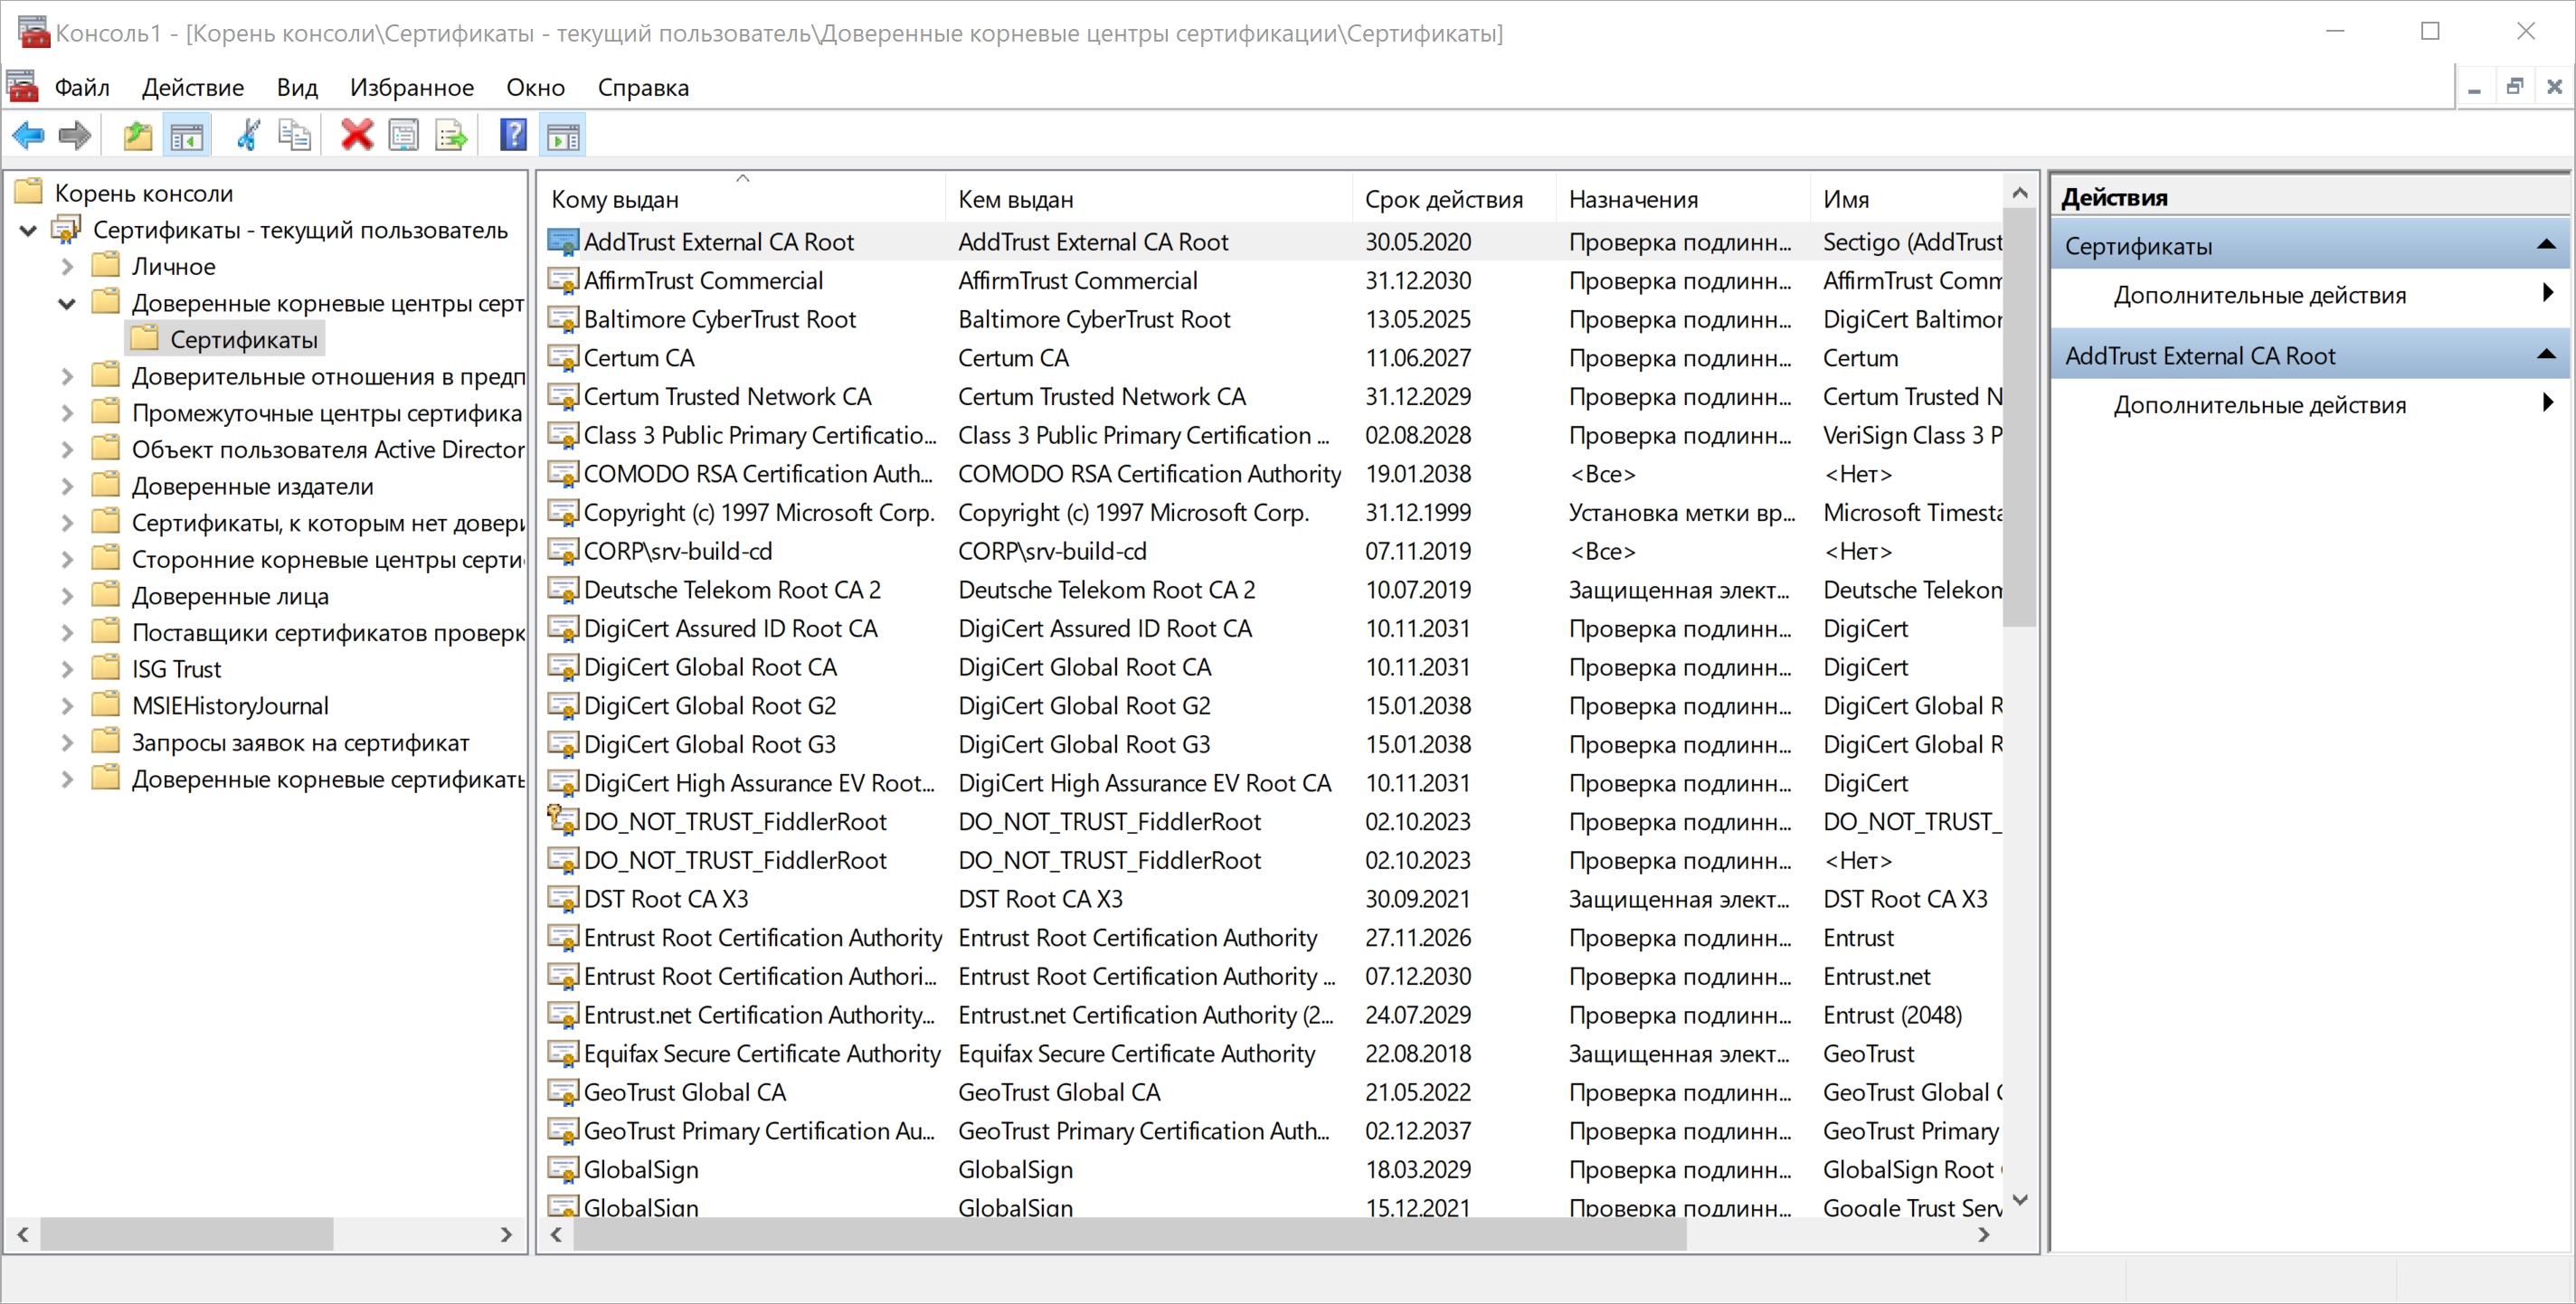
\includegraphics[width=0.95\textwidth]{windowsCertManager.png}
		\end{center}
	\end{frame}

	\begin{frame}[fragile]
		\frametitle{OpenSSL}
		\begin{itemize}
			\item OpenSSL --- библиотека и набор инструментов для криптографии и работы с протоколами SSL/TLS
			\item Стандарт де-факто для работы с открытыми ключами, сертификатами и т.д.
			\item Как сгенерить самоподписанный сертификат:
			
				\begin{minted}{bash}
openssl req -x509 -nodes -days 365 
    -newkey rsa:2048 -keyout privatekey.key 
    -out certificate.crt
				\end{minted}
		\end{itemize}
	\end{frame}

	\section{Аутентификация}

	\subsection{Общий ключ}

	\begin{frame}
		\frametitle{Аутентификация Challenge-Response с общим ключом}
		\begin{center}
			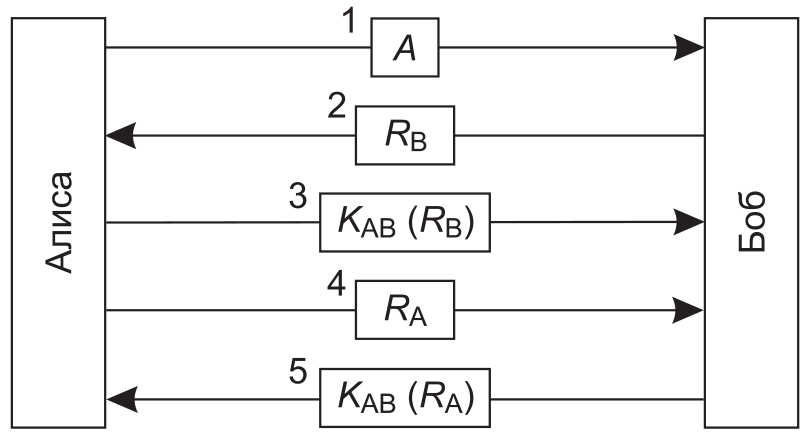
\includegraphics[width=0.5\textwidth]{challengeResponse.png}
			\attribution{Э. Таненбаум}
		\end{center}
		\begin{itemize}
			\item $R_B$ --- \textbf{nonce} (number used once), для предотвращения атаки повтором
			\item $K_{AB}$ --- общий ключ
		\end{itemize}
	\end{frame}

	\begin{frame}
		\frametitle{``Упрощённый'' протокол}
		\begin{center}
			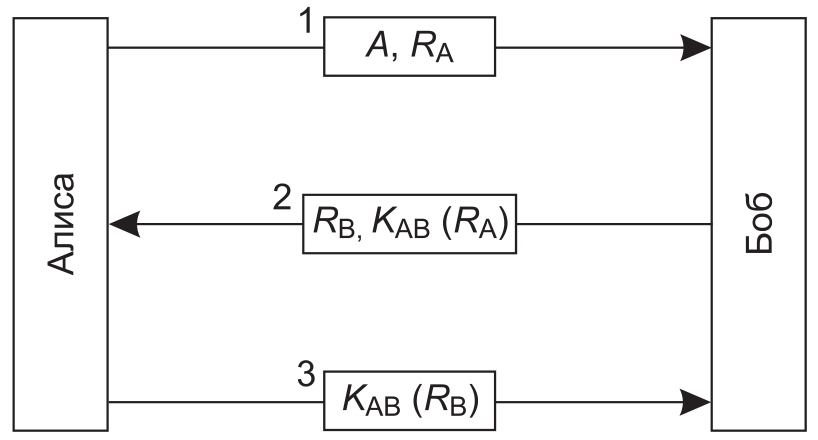
\includegraphics[width=0.5\textwidth]{simpleChallengeResponse.png}
			\attribution{Э. Таненбаум}
		\end{center}
	\end{frame}

	\begin{frame}
		\frametitle{Зеркальная атака}
		\begin{center}
			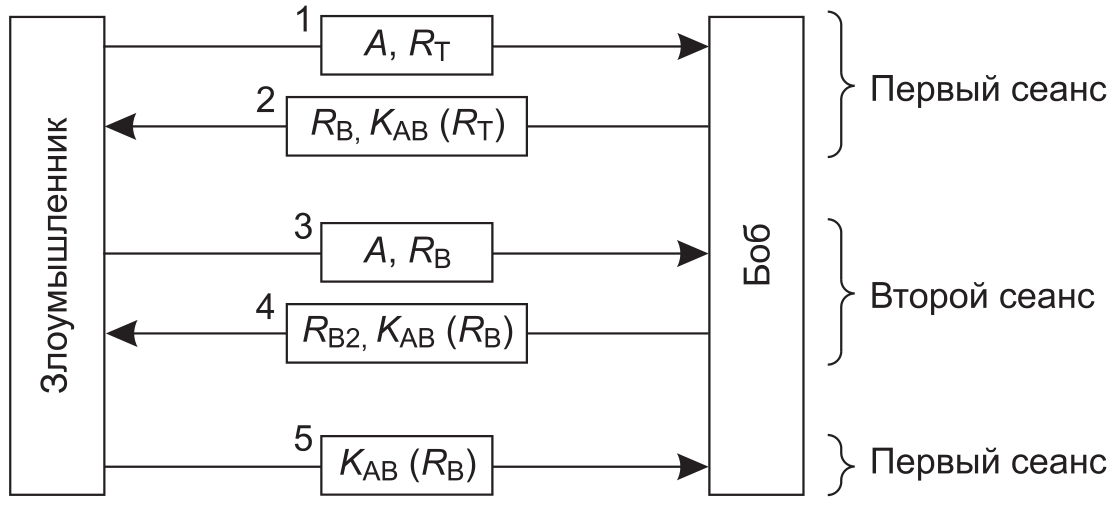
\includegraphics[width=0.65\textwidth]{mirrorAttack.png}
			\attribution{Э. Таненбаум}
		\end{center}
		\vspace{5mm}
		\textbf{Разработать корректный протокол аутентификации сложнее, чем это может показаться}
	\end{frame}

	\begin{frame}
		\frametitle{Правильный протокол}
		\begin{center}
			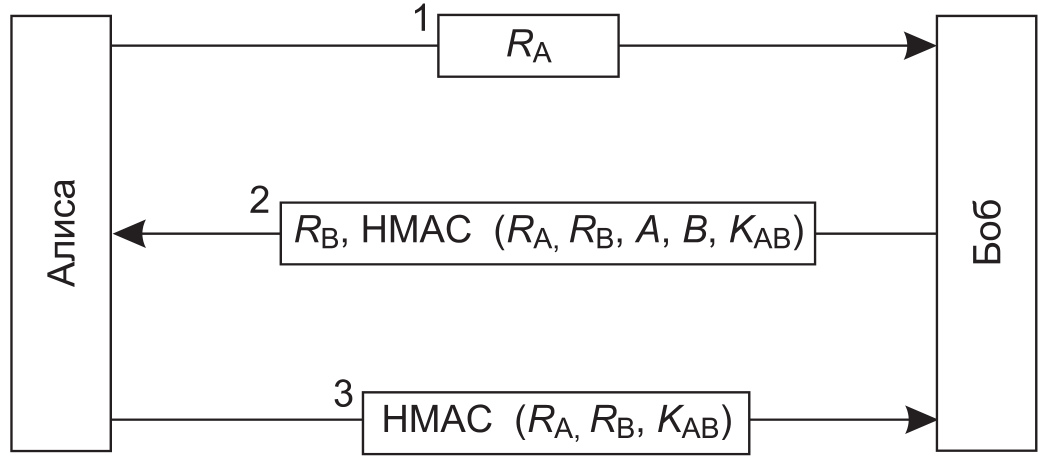
\includegraphics[width=0.6\textwidth]{hmacs.png}
			\attribution{Э. Таненбаум}
		\end{center}
		\begin{itemize}
			\item HMAC --- Hashed Message Authentication Code
		\end{itemize}
	\end{frame}

	\begin{frame}
		\frametitle{Как на самом деле}
		\begin{itemize}
			\item Basic Authentication --- логин и пароль передаются нешифрованными в заголовке HTTP-запроса
			\item HTTPS обеспечивает безопасность
			\item Сервер возвращает Access Token
			\item Access Token предъявляется при каждом следующем запросе
			\begin{itemize}
				\item Имеет ограниченное время жизни, но его можно продлять
			\end{itemize}
			\item Пароли не хранятся на сервере, хранятся их хеши
			\begin{itemize}
				\item Salt --- случайное число, дописываемое к паролю на стороне сервера, хранится вместе с хешем пароля
				\item Если базу паролей украдут, узнать исходные пароли очень сложно
			\end{itemize}
		\end{itemize}
	\end{frame}

	\subsection{Открытый ключ}

	\begin{frame}
		\frametitle{Алгоритм Диффи-Хеллмана}
		\begin{center}
			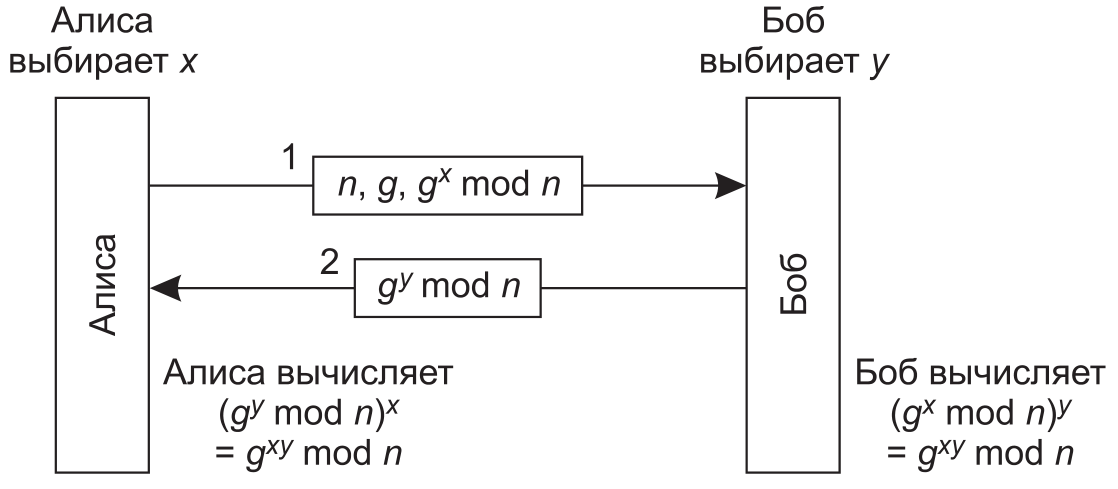
\includegraphics[width=0.6\textwidth]{diffieHellman.png}
			\attribution{Э. Таненбаум}
		\end{center}
	\end{frame}

	\begin{frame}
		\frametitle{Атака ``Man In The Middle''}
		\begin{center}
			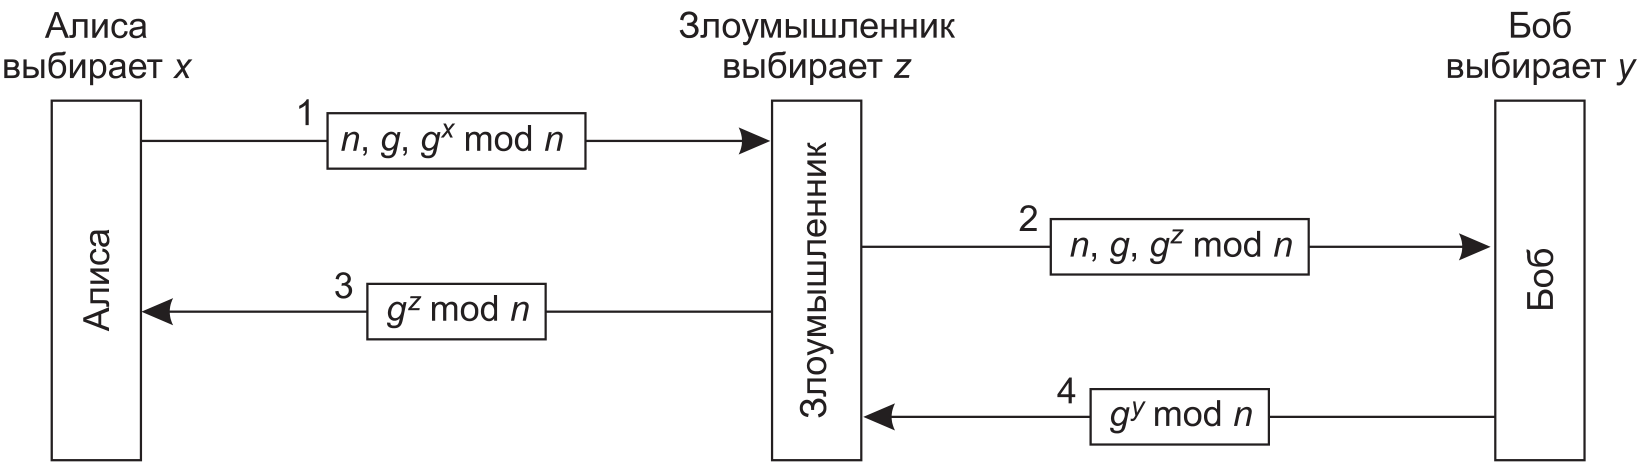
\includegraphics[width=0.9\textwidth]{diffieHellmanMitm.png}
			\attribution{Э. Таненбаум}
		\end{center}
	\end{frame}

	\begin{frame}
		\frametitle{Аутентификация с открытым ключом}
		\begin{center}
			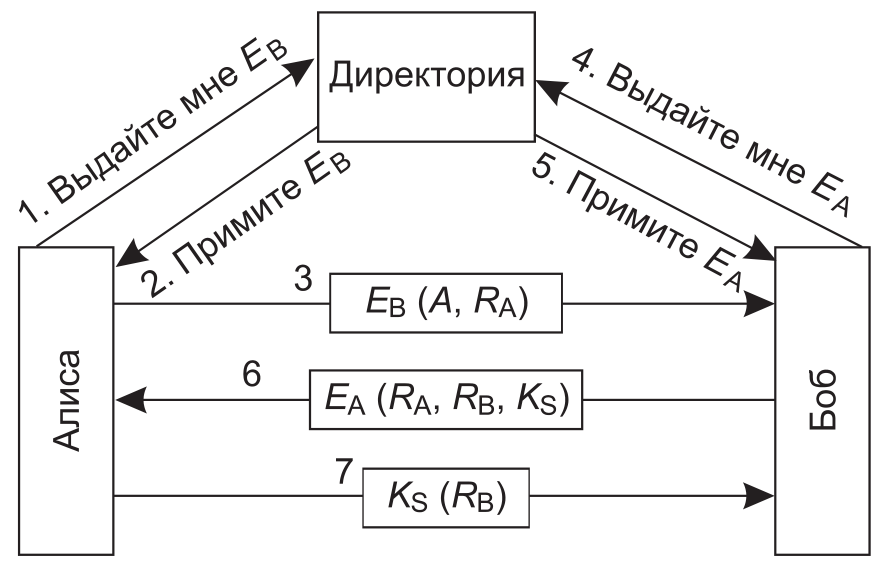
\includegraphics[width=0.6\textwidth]{openKeyAuthentication.png}
			\attribution{Э. Таненбаум}
		\end{center}
		\begin{itemize}
			\item $E_A$, $E_B$ --- открытые ключи Алисы и Боба
			\item $R_A$, $R_B$ --- nonce
		\end{itemize}
	\end{frame}

	\subsection{OAuth2}

	\begin{frame}
		\frametitle{OAuth 2}
		\begin{itemize}
			\item Позволяет разрешить пользование ресурсом, не раскрывая хозяину ресурса логин и пароль пользователя
			\begin{itemize}
				\item Логин по аккаунту в Google или аккаунту в VK
			\end{itemize}
			\item Роли:
			\begin{itemize}
				\item Client --- приложение, пытающееся получить доступ
				\item Resource Server --- сервер, хранящий защищённую информацию. К нему пытается получить доступ клиент
				\item Resource Owner --- пользователь, владеющий защищённой информацией
				\item Authorization Server --- сервер, выдающий клиенту токен на доступ к ресурсному серверу
			\end{itemize}
		\end{itemize}
	\end{frame}

	\begin{frame}
		\frametitle{Протокол}
		\begin{center}
			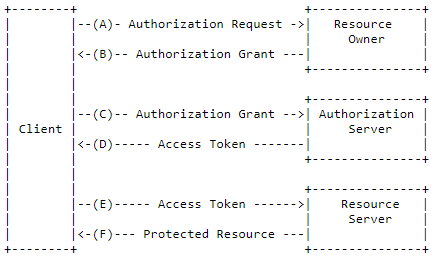
\includegraphics[width=0.5\textwidth]{oauth.png}
			\attribution{RFC 6749}
		\end{center}
	\end{frame}

	\begin{frame}
		\frametitle{Детали}
		\begin{itemize}
			\item Access Token --- выдаётся авторизационным сервером и посылается с каждым запросом, ограниченное время жизни
			\item Refresh Token --- выдаётся авторизационным сервером, используется для получения нового Access Token
			\item Scope --- к какой части ресурса даёт доступ Access Token
		\end{itemize}
	\end{frame}

	\begin{frame}
		\frametitle{Пример: Google OAuth 2.0}
		\begin{columns}
			\begin{column}{0.5\textwidth}
				\begin{itemize}
					\item Google Developer Console, Client ID и Client Secret
					\item Scope
					\item Consent Screen
				\end{itemize}
			\end{column}
			\begin{column}{0.4\textwidth}
				\begin{center}
					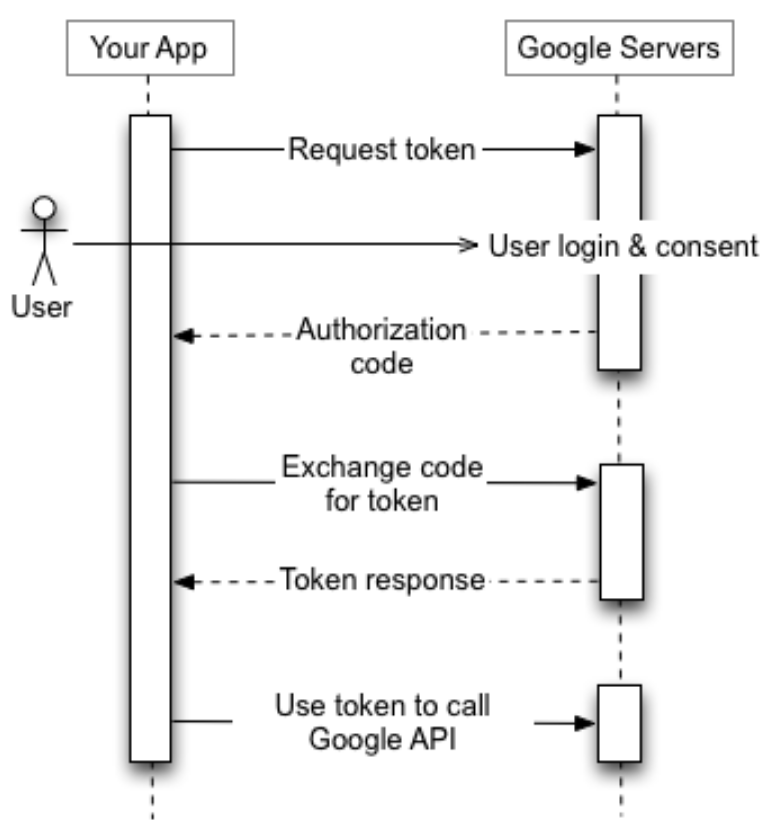
\includegraphics[width=\textwidth]{googleOAuth.png}
					\attribution{\url{https://developers.google.com}}
				\end{center}
			\end{column}
		\end{columns}
	\end{frame}

	\section{Безопасность транспортного уровня}

	\begin{frame}
		\frametitle{HTTPS}
		\begin{center}
			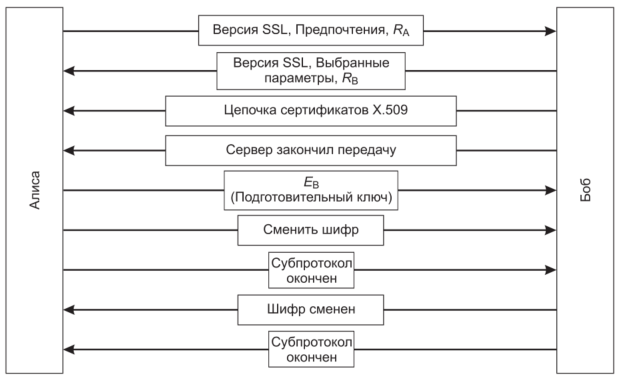
\includegraphics[width=0.6\textwidth]{ssl.png}
			\attribution{Э. Таненбаум}
		\end{center}
		\begin{itemize}
			\item SSL (Secure Sockets Layer)
			\item HTTPS --- HTTP через SSL
			\item Порт 443
			\item Аутентифицируется только сервер
		\end{itemize}
	\end{frame}

	\begin{frame}
		\frametitle{SSL, транспортный субпротокол}
		\begin{center}
			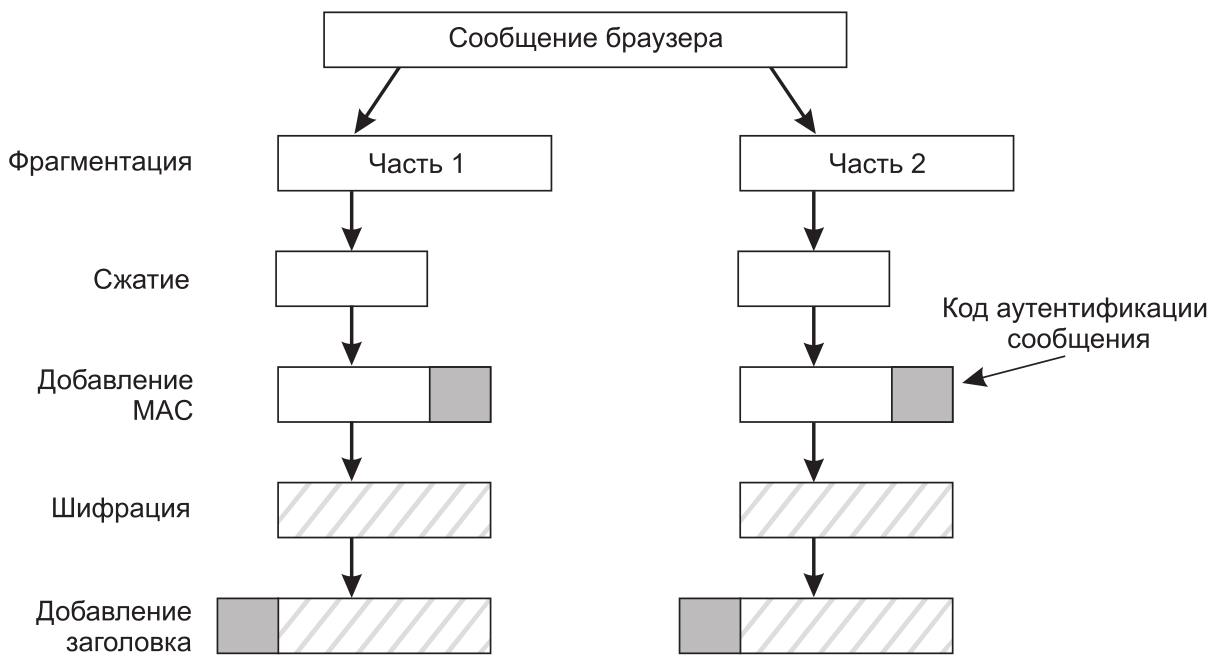
\includegraphics[width=0.6\textwidth]{sslCommunication.png}
			\attribution{Э. Таненбаум}
		\end{center}
		\begin{itemize}
			\item Triple DES + SHA-1
			\item Или RC4 со 128-битным ключом + MD5
			\item TLS --- Transport Layer Security (продвинутый SSL)
		\end{itemize}
	\end{frame}

	\begin{frame}
		\frametitle{DNS Spoofing}
		\begin{columns}
			\begin{column}{0.4\textwidth}
				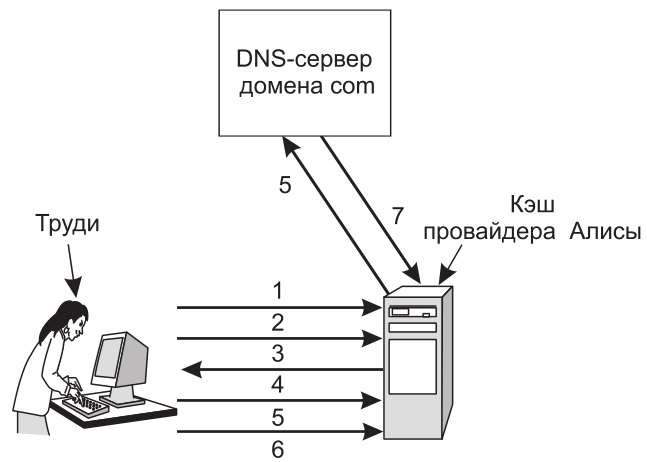
\includegraphics[width=0.95\textwidth]{dnsSpoofing.png}
				\attribution{Э. Таненбаум}
			\end{column}
			\begin{column}{0.6\textwidth}
				\begin{footnotesize}
					\begin{enumerate}
						\item Запрос foobar.trudy-the-intruder.com (чтобы trudy-the-intruder.com попал в кеш провайдера)
						\item Запрос www.trudy-the-intruder.com (чтобы получить следующий порядковый номер провайдера)
						\item Запрос об адресе www.trudy-the-intruder.com к нашему DNS
						\item Запрос к bob.com
						\item Запрос о bob.com к DNS зоны com
						\item Подделанный ответ о bob.com
						\item Настоящий ответ, отвергнутый, потому что уже поздно
					\end{enumerate}
				\end{footnotesize}
			\end{column}
		\end{columns}
	\end{frame}

	\begin{frame}
		\frametitle{Результат}
		\begin{center}
			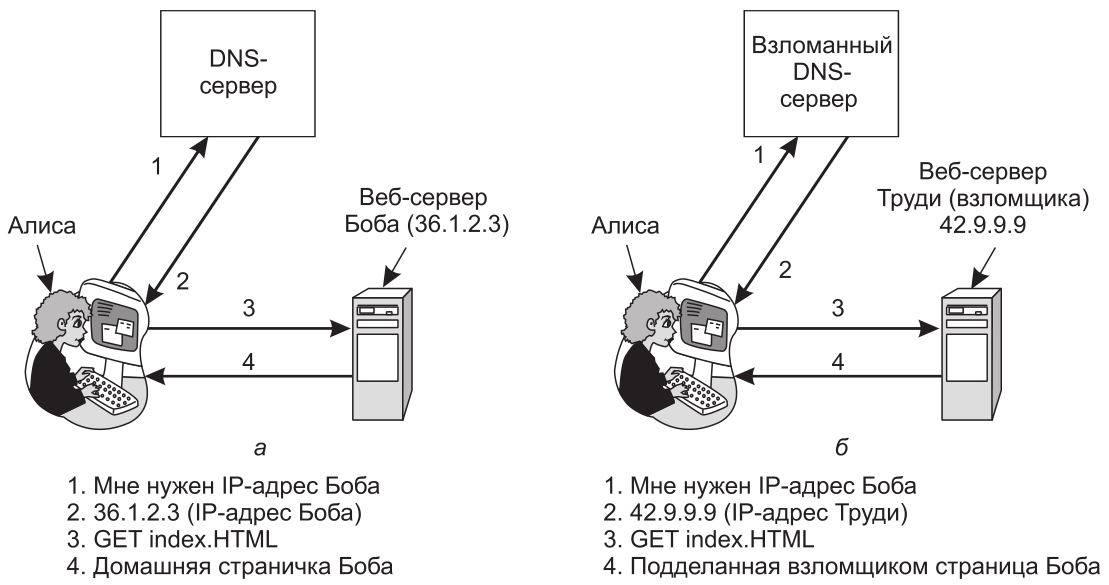
\includegraphics[width=0.9\textwidth]{dnsSpoofingResult.png}
			\attribution{Э. Таненбаум}
		\end{center}
	\end{frame}

	\section{Отладка}

	\begin{frame}
		\frametitle{Как это всё отлаживать}
		\framesubtitle{И ломать}
		\begin{itemize}
			\item Fiddler --- кроссплатфоренный отладочный прокси
			\begin{itemize}
				\item Перехват HTTP-трафика
				\item Man-In-The-Middle-атака с самоподписанными сертификатами
				\begin{itemize}
					\item Расшифровка HTTPS-трафика на лету
				\end{itemize}
				\item Возможность модифицировать HTTP-пакеты, повторять пакеты и т.д.
			\end{itemize}
			\item Wireshark --- когда Fiddler-а мало
			\begin{itemize}
				\item Перехват пакетов на низком уровне
				\item Умеет даже ставить себя как драйвер USB и читать USB-пакеты
			\end{itemize}
		\end{itemize}
	\end{frame}

\end{document}